%%%%%%%%%%%%%%%%%%%%%%%%%%%%%%%%%%%%%%%%%%%%%%%%%%%%%%%%%%%%%%%%%%
%%%%%%%% ICML 2012 EXAMPLE LATEX SUBMISSION FILE %%%%%%%%%%%%%%%%%
%%%%%%%%%%%%%%%%%%%%%%%%%%%%%%%%%%%%%%%%%%%%%%%%%%%%%%%%%%%%%%%%%%

% Use the following line _only_ if you're still using LaTeX 2.09.
%\documentstyle[icml2012,epsf,natbib]{article}
% If you rely on Latex2e packages, like most moden people use this:
\documentclass{article}

% For figures
\usepackage{graphicx} % more modern
%\usepackage{epsfig} % less modern
\usepackage{subfigure}

% For citations
\usepackage{natbib}

% For algorithms
\usepackage{algorithm}
\usepackage{algorithmic}

% As of 2011, we use the hyperref package to produce hyperlinks in the
% resulting PDF.  If this breaks your system, please commend out the
% following usepackage line and replace \usepackage{icml2012} with
% \usepackage[nohyperref]{icml2012} above.
\usepackage{hyperref}

% Packages hyperref and algorithmic misbehave sometimes.  We can fix
% this with the following command.
\newcommand{\theHalgorithm}{\arabic{algorithm}}

% Employ the following version of the ``usepackage'' statement for
% submitting the draft version of the paper for review.  This will set
% the note in the first column to ``Under review.  Do not distribute.''
%\usepackage{icml2012}
% Employ this version of the ``usepackage'' statement after the paper has
% been accepted, when creating the final version.  This will set the
% note in the first column to ``Appearing in''
\usepackage[accepted]{icml2012}


% The \icmltitle you define below is probably too long as a header.
% Therefore, a short form for the running title is supplied here:
\icmltitlerunning{Weather Forecasting using Probabilistic Graphical Models}

\begin{document} 

\twocolumn[
\icmltitle{Weather Forecasting using Probabilistic Graphical Models}

% It is OKAY to include author information, even for blind
% submissions: the style file will automatically remove it for you
% unless you've provided the [accepted] option to the icml2012
% package.
\icmlauthor{Felipe Hern\'andez}{felipeh@andrew.cmu.edu}
\icmladdress{Depertment of Civil and Environmental Engineering, University of Pittsburgh}
\icmlauthor{Amos Ng}{ajng@andrew.cmu.edu}
\icmladdress{Language Technologies Institute, Carnegie Mellon University}

% You may provide any keywords that you 
% find helpful for describing your paper; these are used to populate 
% the "keywords" metadata in the PDF but will not be shown in the document
\icmlkeywords{boring formatting information, machine learning, ICML}

\vskip 0.3in
]

\begin{abstract} 
Weather prediction has usually involved running physical models of weather
phenomena in order to predict future conditions. In this project, instead of
focusing on the physics, we propose using probabilistic models based on
meteorological observations gathered by NASA to produce future weather
conditions.
\end{abstract} 

\section{Introduction}
\label{submission}

Weather forecasting is used for a broad range of purposes, ranging from personal
activity planning to large-scale economic decision-making to emergency
preparation and response. The availability and the accuracy of forecasts thus
have a profound impact on human activities at many levels, both in measurable and
unmeasurable aspects.

However, predicting weather is a difficult research problem. Most often,
physically-based models with global and regional scales are used to forecast
future conditions. In this project, we will instead take a probabilistic machine
learning approach focused on a regional scale and predict atmospheric variables
at specific geographic locations. As opposed to deterministic methods, this
probabilistic approach will help us not only estimate the most probable values
for the forecasting variables as a regression approach would, but also determine
what is the level of uncertainty associated with each forecasted variable.
Uncertainty becomes more important as the forecasting time period becomes
larger. This additional knowledge would be key for potential users in order to
assess how much they can trust the delivered forecasts.

The forecasts will be based on prior atmospheric states in the neighborhood of
the selected location. In particular, we will attempt to predict the probability
distributions of variables such as pressure, precipitation, and temperature
based on data recorded by NASA using assimilated land products.

\section{Related work} 
 
Researchers in the atmospheric sciences have investigated a variety of methods
for weather forecasting. Many subtle physical phenomena affect the weather at
any given time, including energy and mass fluxes between the sun and different
layers of the atmosphere, ground, and ocean. In order for these phenomena
to be modelled, physically-based equations need to be used to simulate each of
the mass and energy exchanges between the finite volumes that make up the
domain. Machine learning approaches have been explored to construct simplified
models based on atmospheric measurements, but are not very popular among
meteorologists.

Many of these techniques are tailored to fit the nature of the observations
available. Weather monitoring stations are the predominant data source,
providing point measurements with high accuracy and varying temporal resolution.
Artificial neural networks (ANN) have proven to be effective in such cases for
forecasting rainfall amounts in the near future given a time series of
previously observed values, as in the early work of \citet{French1992}. The work
by \citet{maier2000} presents an overview of such works using ANN.

More recent works have attempted to combine ANNs with other techniques to
improve the performance of predictions. In \cite{hong2008}, a recursive ANN is
trained using a support vector regression together with a chaotic particle swarm
optimizer: the particle swarm optimization meta-heuristic is used to find the
optimum parameters of the support vector regression model leading to a better
performance when compared to other ANNs. Similarly, a genetic algorithm is used
to perform the calibration of the network in \cite{nasseri2008}, given that the
defining of the weights between the network's neurons is a non-convex
optimization problem.

A related method is presented by \citet{Partal2007}, where
the results from discrete wavelet transforms over the training data are fed into
a neuro-fuzzy model for prediction. Wavelet neuro-fuzzy approaches are also
studied by \citet{Kisi2011} and contrasted with single neuro-fuzzy models,
single genetic programming regressions, and their conjoint counterparts using
wavelet transformations. Algorithms of different nature than ANNs that are used
in weather forecasting include linear regression, discriminant analysis, and
logistic regression as reviewed in the work by \citet{applequist2002}.

Recently, meteorological observations from land-based and satellite-based
Doppler radars have become widely available, providing enhanced coverage at
the cost of decreased precision. These sources of information add a spatial
dimensions to the forecasting problem. Fourier spectrum, structure function,
and moment-scale analyses are used to understand radar precipitation in
\cite{harris2007}; decision trees are used on a Lagrangian reference framework
to learn rainfall behavior from satellite images in \cite{Yang2007}; and and
several sources of information, including satellite and radar images, are
proposed in \cite{Bartok2010} for the spatial estimation of multiple weather
variables.

Forecasting models have also been created to take advantage
of interdependencies between atmospheric variables that are estimated,
instead of being measured, through the use of other models. For
example, rain-gauge data and outputs from atmospheric models are used for
forecasting precipitation in \cite{kuligowski1998} and \cite{ramirez2005}.
Additional upper air soundings are also used in \cite{Hall1999}, and radar and
satellite data is incorporated into forecasts in \cite{Koizumi1999}.

\section{Data collection}

As mentioned previously, there are multiple sources of meteorological
information available online. Usually these sources are provided by government
agencies such as NOAA and NASA, and have different levels of post-processing of
raw data from gauges, land radars, and satellites.

The North American Land Data Assimilation System (NLDAS), a service hosted by
the Goddard Earth Sciences Data and Information Services Center at NASA, is a
multi-variable source of information produced through the assimilation of land
measurements. We will focus mainly on this dataset due to both its relative high
precision and the multiple variables it reports: precipitation, atmospheric
pressure, humidity, temperature, wind speed, convective potential energy, and
radiation flux.

The NLDAS product provides hourly weather data for the US beginning in 1980.
Each sampled time in the data set includes the following values per cell in a
grid of resolution 1/8 of a degree in both latitude and longitude directions.
Figure~\ref{fig:example_rainfall} provides an illustration of one such hour-long
sample. Table~\ref{tab:variables} lists the full set of variables available at
each spatial cell.

\begin{figure}[ht] \vskip 0.2in
\begin{center}
\centerline{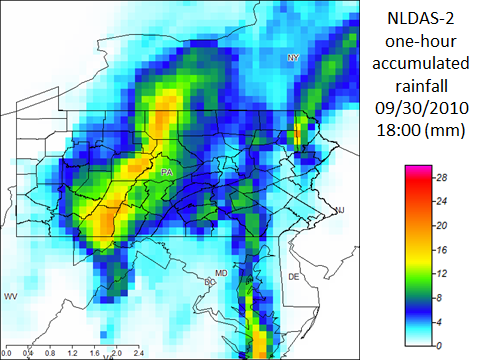
\includegraphics[width=0.9\columnwidth]{images/weather.png}}
\caption{This is one example of a rainfall image produced during a severe storm in Pennsylvania in 2010. Each cell in this image has a size of roughly 10 km $\times$ 10 km. More information on the NLDAS-2 data products can be found on the following URLs: \url{http://ldas.gsfc.nasa.gov/index.php} and \url{http://disc.sci.gsfc.nasa.gov/hydrology/data-holdings}.}
\label{fig:example_rainfall}
\end{center}
\vskip -0.2in
\end{figure}

\begin{table*}[t]
\caption{Meteorological variables available on NLDAS-2}
\label{tab:variables}
\begin{tabular}{p{4cm} p{8cm} p{3.5cm}}
\hline
\textbf{Name} &\textbf{Description} &\textbf{Units} \\
\hline
precipitation &Accumulated height of precipitated water column &millimeters\\
available potential energy &180-0 mb above ground Convective Potential
Energy &Joules per kilogram \\
\% convective precipitation &Fraction of total precipitation that is convective
&none \\
LW radiation &Long wave radiation flux downwards (surface) &watts per square
meter \\
SW radiation &Short wave radiation flux downwards (surface) &watts per
square meter \\
potential evaporation &Potential evaporation &millimeters \\
surface pressure &Surface pressure &pascals \\
specific humidity &2 m above ground Specific humidity &none \\
temperature 2 m &2 m above ground Temperature &kelvin \\
zonal wind speed &10 m above ground Zonal wind speed &meters per second \\
meridional wind speed &10 m above ground Meridional wind speed &meters per
second \\
\hline
\end{tabular}
\end{table*}

\section{Methods}

The task of forecasting weather states using the NLDAS-2 dataset can be
approached by attempting to estimate the maps for each variable one hour into
the future given the current state maps and, optionally, additional previous
maps. These maps can be obtained by estimating the values for each cell in the
raster one by one. This strategy effectively divides the problem into a
large set of easier sub-problems that can be more easily addressed. By
estimating each value one time step into the future, longer forecasts can be
made by applying the same strategy iteratively on the next time step. This, of
course, would mean an increase in the uncertainty.

Let $X_k^{i,j,t}$ denote variable $k$ at time step $t$ at coordinates $i, j$.
The estimation procedure would rely on a model $f(\cdot)$ that is able to
compute the conditional probability of a variable $X$ given a set of observations
$\hat{X}$ that belong to a spatial frame $S$ and a temporal frame $T$:

\begin{equation}
\label{eq:condProb}
P(X) = f[\{X_k^{i,j,t}\} | (i,j) \in S, t \in T]
\end{equation}

There are several alternatives for determining which variables to use as inputs
of $f(\cdot)$. Some of the alternatives are listed below. Figure
\ref{fig:plate_models} shows the graphical models for each of these cases.

\begin{enumerate}
\item Values on time $t + 1$ depend on the values of all variables of the same
cell on time step $t$
\item Values on time $t + 1$ depend on the values of all variables of the same
cell on time step $t$ and time step $t - 1$ (and maybe time step $t- 2$). We
could use the time derivatives to account for these temporal variations.
\item Values on time $t + 1$ depend on the values of all variables on the
vicinity of the cell at time step $t$. We could account for these spatial
variations by using spatial gradients.
\item Values on time $t + 1$ depend on the values of all variables on the
vicinity of the cell at time step $t$ and time step $t -1$. This option includes
both temporal and spatial derivatives.
\end{enumerate}

\begin{center}
\begin{figure}
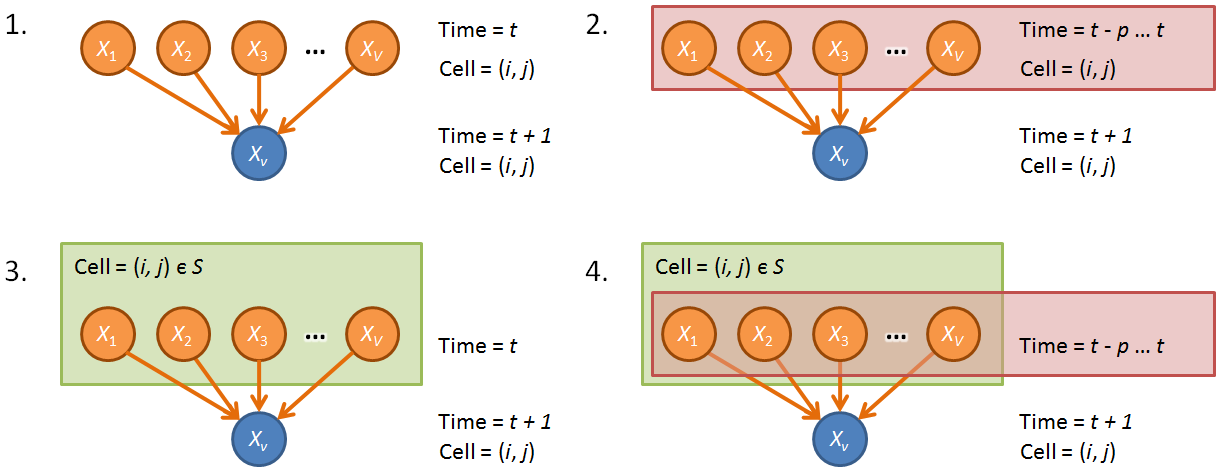
\includegraphics[width=0.9\columnwidth]{images/plate_models.png}
\caption{Graphical models to represent different
selections of input variables for the predictive model. \textit{S} represents
a set of neighboring cells and \textit{p} represents the number of previous
time steps to use in addition to time step \textit{t}. 1.
Local dynamic; 2. Local with extended time dependency; 3.
Neighborhood dynamic; 4. Neighborhood with extended time
dependency.}\label{fig:plate_models}
\end{figure}
\end{center}

We chose to model the joint probability distribution of the variables using
Gaussian Graphical Models (GGM) also known as Gaussian Markov Random Fields
(GMRF). These models are multi-variable Gaussian probability distributions with
the particularity that the dependencies between the random variables are
purposefully kept to a minimum. This sparsity allows to create graphical
representations that are meaningful to the users, and to run inference
algorithms with reduced computational requirements. In GGM the density function
of the variable vector $X$ is computed using a mean vector $\mu$ and a
covariance matrix $\Sigma$ using the following expression:

\begin{equation}
\label{eq:gaussian}
P(X|\mu,\Sigma) =
\frac{1}{(2\pi)^{n/2}\vert\Sigma\vert^{1/2}}\exp[-\frac{1}{2}(X - \mu)^T\Sigma^{-1}(X - \mu)]
\end{equation}

Sparsity in GGMs can be achieved by using regularized linear regressions like
the lasso \cite{tibshirani1996} to estimate the coefficients of the precision
matrices $\Omega=\Sigma^{-1}$. The precision matrix has coefficients with a
value of zero for pairs of variables that are conditionally independent. Two
algorithms that apply this technique for the estimation of the precision matrix
are the neighborhood estimation \cite{meinshausen2006} and the graphical lasso
(glasso - \cite{Friedman2008}). We used glasso for the purposes of this project.

Once we have learned the GGM, we can use inference to perform the forecasting.
Inference implies finding the conditional distributions of all the unknown or
unobserved variables ($X^{\{1\}}$) given the known or observed variables
($X^{\{2\}} = o$). So for example we may want to determine the values of the
variables a time $t + 1$ given the observations at time $t$: $P(X^{t+1} | X^t
= o)$. The conditional distribution is also a multi-variate Gaussian
distribution which can be obtained using a na\"ive matrix inversion approach
described in \cite{Koller2009}: let $\mu_1$ be the vector of mean values of the
unobserved variables, and $\mu_2$ the means of the observed variables.
Similarly, let $\Sigma_{11}$ be the part of the covariance matrix $\Sigma$ with
the covariances between unobserved variables, $\Sigma_{12}$ and $\Sigma_{21}$
with the covariates between unobserved and observed variables, and $\Sigma_{22}$
with the covariates between observed variables. $\mu$ and $\Sigma$ are thus
partitioned as:

\begin{equation}
\label{eq:distPartition}
\mu = \left( \begin{array}{ccc}
\mu_1 \\ \mu_2 
\end{array} \right),
\Sigma = \left( \begin{array}{ccc}
\Sigma_{11} & \Sigma_{12} \\
\Sigma_{21} & \Sigma_{22}
\end{array}\right)
\end{equation}

With this partition we can compute the mean ($\hat\mu$) and the covariance
matrix ($\hat\Sigma$) of the conditional distribution:

\begin{eqnarray}
\label{eq:naiveInference1}
P(X^{\{1\}} | X^{\{2\}} = o) \sim \mathcal{N}(\hat\mu, \hat\Sigma) \\
\label{eq:naiveInference2}
\hat\mu = \mu_1 + \Sigma_{12}\Sigma_{22}^{-1}(o - \mu_2) \\
\label{eq:naiveInference3}
\hat\Sigma = \Sigma_{11} - \Sigma_{12}\Sigma_{22}^{-1}\Sigma_{21}
\end{eqnarray}

This na\"ive approach requires inverting a matrix, an operation which has a
complexity of $\mathcal{O}(n^3)$. This operation becomes too expensive with
large models and thus more efficient methods become necessary in these cases.
Taking advantage of the graphical structure of the GGM, observed variables can
be eliminated one at a time in an given order so as to minimize the size of the
resulting intermediate terms. This operation marginalizes out each observed
variable until a conditional distribution with only the unobserved variables
remains. In this way, the size of the covariance matrices that are used to
define the intermediate distributions is effectively reduced and so are the
computational requirementes.

This is the principle behind the belief propagation algorithm \cite{Koller2009},
which consists in a series of variable eliminations resulting in a set of
messages. These messages are marginalized conditional distributions that are
passed between the nodes of the graph so that the conditional distributions at
each sub-graph can be easily computed. In the case of GGM, variable elimination
consists in performing Gaussian elimination on the probability
distribution of the cliques. The probability distribution of a clique is
a multi-variate Gaussian distribution whose parameters are given by the
elements of the mean vector $\mu$ and the covariance matrix $\Sigma$ that
correspond to the variables in the clique. Variable elimination is performed by
using equations \ref{eq:naiveInference1}, \ref{eq:naiveInference2}, and
\ref{eq:naiveInference3} \cite{malioutov2008approximate}.

However, when the graph contains cycles, it is not possible to perform the
elimination in such a way that all possible dependency paths are considered
simultaneously. Loopy belief propagation \cite{murphy1999} consists in extending
the message passing algorithm to graphical models with cycles.
Although no exact results are obtained, the approximate solutions provided are
good enough in a wide spectrum of cases. Variations of the loopy belief
propagation algorithm exists that look to improve its performance and
scalability. They focus on walking sums that can be used to speed up convergence
at the cost of accuracy, and on the construction of low-rank aliasing matrices
to approximate the inversion of the covariance matrix from the presicion matrix
\cite{malioutov2008approximate}.

\section{Results}

Thus far we have downloaded the data from the above links, over the range of a
one month for an area around Pittsurgh of size 60 km $\times$ 60 km. We put the
data into a database for efficient storage and retrieval. We then preprocessed the
data to be arranged in a series of training examples arranged in the four cases
mentioned before. We then used glasso to obtain the precision matrix for
relations between the various variables in the data.

The results for different glasso regularization parameters are plotted in
Figures~\ref{fig:data_0} to \ref{fig:data_100}. We also ran glasso to infer the
network structure for variables in both $t$ and $t - 1$ timestamps; results are
shown in Figures~\ref{fig:dynamic_0} to \ref{fig:dynamic_100}. Finally, we ran
glasso to infer the relationships between the various states of weather and the
changes from one state to the other. Results for this are shown in Figures~
\ref{fig:grad_0} to \ref{fig:grad_100}.

\begin{figure}
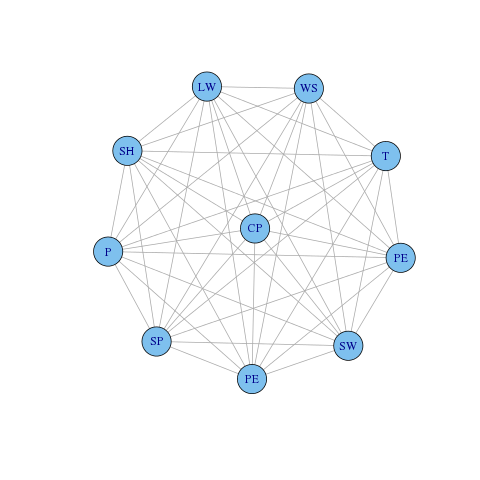
\includegraphics[width=0.9\columnwidth]{images/data_0.png}
\caption{Network structure as inferred from the precision matrix obtained from results thus far, using a GLASSO regularization parameter of 0 (equivalent to no regularization). Edges are shown where precision matrix entries were nonzero.}
\label{fig:data_0}
\end{figure}

\begin{figure}
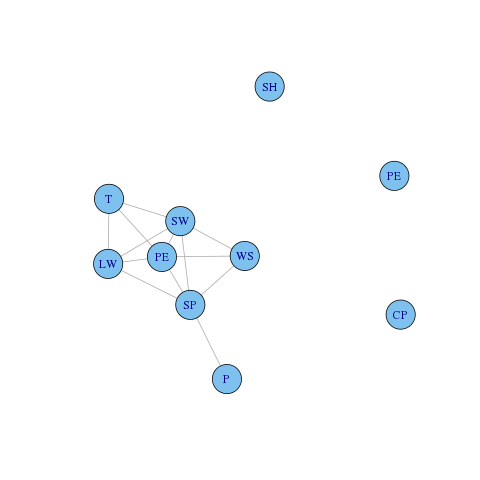
\includegraphics[width=0.9\columnwidth]{images/data_50.png}
\caption{Network structure with a GLASSO regularization parameter of 50.}
\label{fig:data_50}
\end{figure}

\begin{figure}
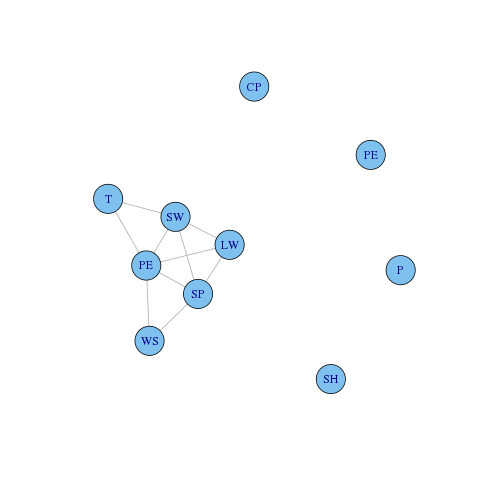
\includegraphics[width=0.9\columnwidth]{images/data_100.png}
\caption{Network structure with a GLASSO regularization parameter of 100.}
\label{fig:data_100}
\end{figure}

\begin{figure}
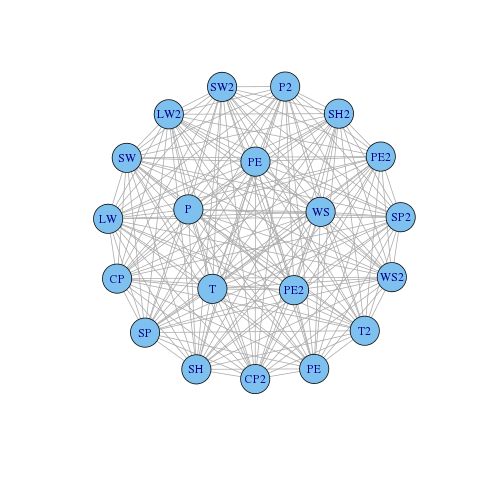
\includegraphics[width=0.9\columnwidth]{images/dynamic_0.png}
\caption{Network structure of dynamic data with a GLASSO regularization parameter of 0 (no regularization).}
\label{fig:dynamic_0}
\end{figure}

\begin{figure}
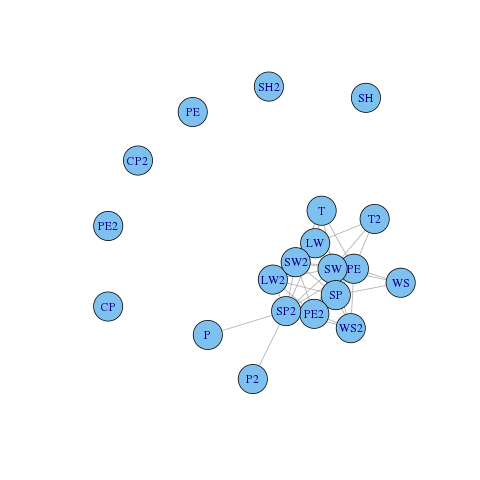
\includegraphics[width=0.9\columnwidth]{images/dynamic_50.png}
\caption{Network structure of dynamic data with a GLASSO regularization parameter of 50.}
\label{fig:dynamic_50}
\end{figure}

\begin{figure}
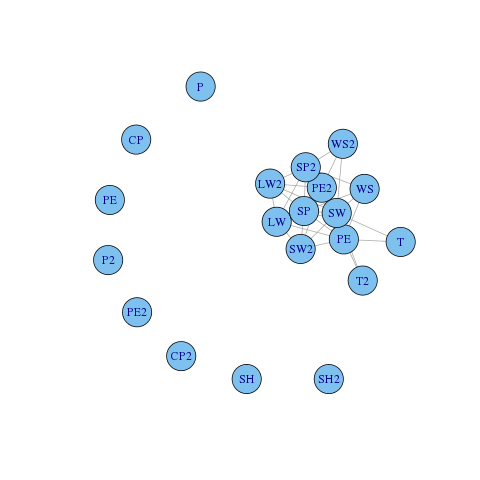
\includegraphics[width=0.9\columnwidth]{images/dynamic_100.png}
\caption{Network structure of dynamic data with a GLASSO regularization parameter of 100.}
\label{fig:dynamic_100}
\end{figure}

\begin{figure}
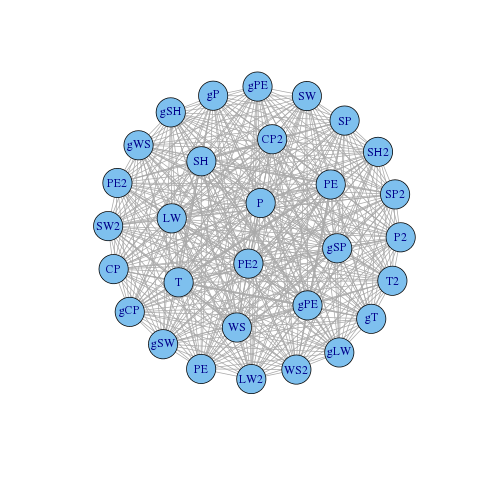
\includegraphics[width=0.9\columnwidth]{images/grad_0.png}
\caption{Network structure of gradient data with a GLASSO regularization parameter of 0 (no regularization).}
\label{fig:grad_0}
\end{figure}

\begin{figure}
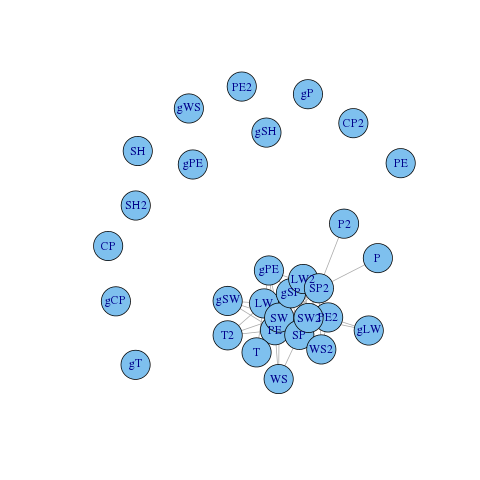
\includegraphics[width=0.9\columnwidth]{images/grad_50.png}
\caption{Network structure of gradient data with a GLASSO regularization parameter of 50.}
\label{fig:grad_50}
\end{figure}

\begin{figure}
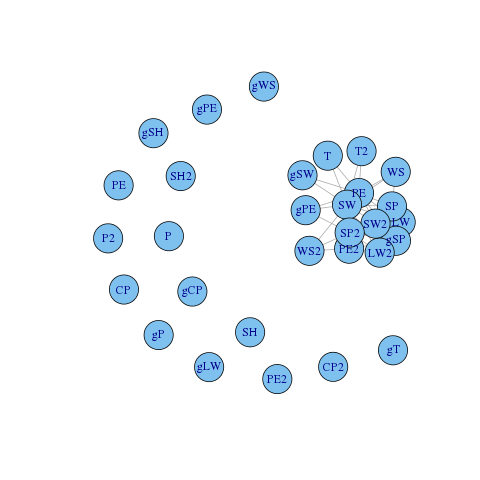
\includegraphics[width=0.9\columnwidth]{images/grad_100.png}
\caption{Network structure of gradient data with a GLASSO regularization parameter of 100.}
\label{fig:grad_100}
\end{figure}

\section{Activity plan}

We plan to use different probabilistic graphical models (HMMs, CRFs, plain old
Bayesian networks) to try to learn the conditional probability distribution
parameters of weather variables maps given the observed values from previous
time steps. We are currently assuming the distributions to take on a Gaussian
form, and learning the distributions from scratch.

\subsection{Old Activities}
The old list of activities that we had intended to perform include
\begin{enumerate}
\item Selection of the dataset and the study area
\item Data download and pre-processing
\item Variable discretization strategy
\item Na\"\i ve Bayes formulation
\item Review of probabilistic graphical models for continuous variables
\end{enumerate}

\subsection{New Activities}
The new list of activities we intend to perform are
\begin{enumerate}
\item Formulation of data in other commonly-used graphical models (CRFs, HMMs, etc.).
\item Cross-validation to check for model accuracy while preventing overfitting
\end{enumerate}

\bibliography{bibliography}
\bibliographystyle{icml2012}

\end{document}


% This document was modified from the file originally made available by
% Pat Langley and Andrea Danyluk for ICML-2K. This version was
% created by Lise Getoor and Tobias Scheffer, it was slightly modified  
% from the 2010 version by Thorsten Joachims & Johannes Fuernkranz, 
% slightly modified from the 2009 version by Kiri Wagstaff and 
% Sam Roweis's 2008 version, which is slightly modified from 
% Prasad Tadepalli's 2007 version which is a lightly 
% changed version of the previous year's version by Andrew Moore, 
% which was in turn edited from those of Kristian Kersting and 
% Codrina Lauth. Alex Smola contributed to the algorithmic style files.  



